\documentclass[12pt,a4paper,bahasa]{article}
\usepackage{graphicx}



\begin{document}

\title{LAPORAN DATABASE}   
\maketitle

\textbf{Kartu Tanda Penduduk (KTP) } adalah identitas resmi Penduduk sebagai bukti diri yang diterbitkan oleh Instansi Pelaksana yang berlaku di seluruh wilayah Negara Kesatuan Republik Indonesia. Kartu ini wajib dimiliki Warga Negara Indonesia (WNI) dan Warga Negara Asing (WNA) yang memiliki Izin Tinggal Tetap (ITAP) yang sudah berumur 17 tahun atau sudah pernah kawin atau telah kawin. \\

Proses Bisnis KTP.\\

Kartu Tanda Penduduk adalah identitas resmi penduduk sebagai bukti diri yang diterbitkan oleh Instansi Pelaksana yang berlaku di seluruh wilayah Negara Kesatuan Republik Indonesia. Kartu ini wajib dimiliki oleh Warga Negara Indonesia danWarga Negara Asing yang memiliki izin tetap tinggal, berumur 17 tahun, sudah pernah kawin atau telah kawin. Anak dari orang tua yang memiliki izin tetap tinggal serta telah berusia 17 tahun dan memiliki KTP.  KTP bagi WNI ini berlaku selama 5   tahun dan tanggal berakhirnya disesuaikan dengan tanggal dan bulan kelahiran yang bersangkutan dan KTP menurut WNA berlaku dengan izin tetap tinggal. Untuk warga yang berusia 60 tahun ke atas mendapat KTP seumur hidup yang tidak perlu diperpanjang selama setiap lima tahun sekali.\\

Pembuatan Kartu Tanda Penduduk (E-KTP)\\

       Syarat pembuatan KTP baru sebagai berikut:\\
       \begin{enumerate}
       \item Telah berusia 17 tahun , sudah kawin atau pernah kawin.
       \item Fotokopi KK, jadi pada dasarnya untuk pembuatan baru hanya membawa fotokopi KK.
       \item Surat pengantar dari RT/RW. 
       \end{enumerate}

Syaratpembuatan KTP bagi orang asing yang punya izin tetap://
	\begin{enumerate}
	\item Surat keterangan kehilangan dari kepolisian(jika 		   kasusnya KTP anda hilang).
	\item KTP yang rusak(jika kasusnya KTP anda rusak).
	\item Fotocopy KK.
	\item Dokumen perjalanan RI atau dokumen perjalanan(jika anda orang asing).
	\item Kartu izin tinggal tetap(jika anda orang asing).
	\end{enumerate}
	
	Atribut KTP:\\
	\begin{enumerate}
	\item NIK
	\item Nama Lengkap
	\item TempatdanTanggalLahir
	\item JenisKelamin
	\item Agama 
	\item Status
	\item GolonganDarah
	\item AlamatLengkap(RT,RW,Kelurahan, danKecamatan)
	\item Agama
	\item Status Perkawinan
	\item Pekerjaan
	\item Kewarganegaraan
	\item BerlakuHingga
	\item Pas Foto
	\item Tempatdantanggaldikeluarkannya KTP
	\item TandaTanganpemegang KTP
	\end{enumerate}
	
	\textbf{Normalisasi Tabel}
	\begin{enumerate}
	
	\item Tabel Universal\\
	
\begin{figure}[!htbp]
\centering
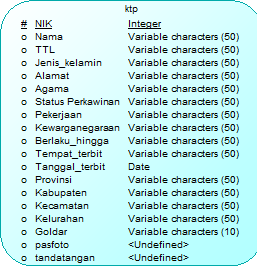
\includegraphics[scale=1.5]{gambar/universal.png}
\caption{\textit{universal}}
\label{univ}
\end{figure}	
	
	Dari proses bisnis yang telah diberikan tersebut didapatkan tabel universal dengan atribut yang ada di tabel di atas.
	
	\item Tabel Kependudukan\\
	
\begin{figure}[!htbp]
\centering
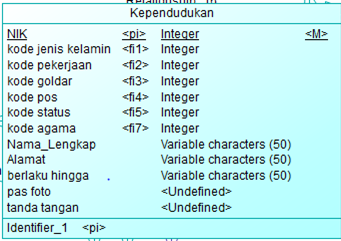
\includegraphics[scale=1.5]{gambar/kependudukan.png}
\caption{\textit{kependudukan}}
\label{kependudukan}
\end{figure}	
	
	Ialah tabel yang berisikan identitas resmi seorang WNI yang terdiri atas kode unik NIK yang berperan sebagai primary key dari tiap atribut yang ada. Tabel kependudukan ini berisikan foreign key yang merupakan primaty key dari tabel jeniskelamin, tabel pekerjaan, tabel golongan darah, tabel kodepos, tabel statusperkawinan, dan tabel agama.
	
	\item Tabel Agama\\
	
\begin{figure}[!htbp]
\centering
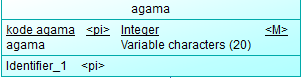
\includegraphics[scale=1.5]{gambar/agama.png}
\caption{\textit{agama}}
\label{agama}
\end{figure}
	
	Dari tabel agama tersebut, berisikan atribut kodeagama sebagai primary key dengan tipe data integer dengan atribut lain ialah agama dengan tipe data yang digunakan  ialah varchar.
	
	\item Tabel Status Perkawinan\\
\begin{figure}[!htbp]
\centering
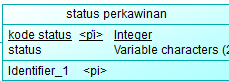
\includegraphics[scale=1.5]{gambar/status.png}
\caption{\textit{status}}
\label{status}
\end{figure}
	
	Dari tabel status perkawinan tersebut, didapatkan kodestatus dengan tipe data integer yang berperan sebagai primary key dari atribut yang lainnya yaitu atribut status dengan tipe data variable character
	
	\item Tabel Goldar\\
\begin{figure}[!htbp]
\centering
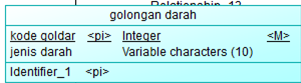
\includegraphics[scale=1.5]{gambar/goldar.png}
\caption{\textit{goldar}}
\label{goldar}
\end{figure}
	
	Dari tabel golongan darah tersebut, terdapat atribut kodegoldar dengan tipe data integer sebagai primary key dan atribut lainnya yaitu jenisdarah yang memiliki tipe data variable character.
	\item Tabel Pekerjaan\\
\begin{figure}[!htbp]
\centering
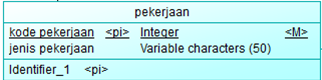
\includegraphics[scale=1.5]{gambar/pekerjaan.png}
\caption{\textit{pekerjaan}}
\label{perkerjaan}
\end{figure}


Dari tabel tersebut didapatkan  kodepekerjaan yang berperan sebagai primary key dengan tipe data integer dan jenis pekerjaan yang memiliki tipe data variable character.

	\item Tabel Jeniskelamin\\
\begin{figure}[!htbp]
\centering
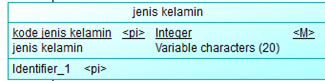
\includegraphics[scale=1.5]{gambar/jeniskelamin.png}
\caption{\textit{jeniskelamin}}
\label{jeniskelamin}
\end{figure}	

Dari tabel jenis kelamin tersebut, didapatkan atribut kodejeniskelamin yang berfungsi sebagai primary key dari tabel tersebut dengan tipe data integer dan atribut jeniskelamin yang memiliki tipe data variable character.

	\item Tabel Kode pos\\
\begin{figure}[!htbp]
\centering
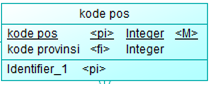
\includegraphics[scale=1.5]{gambar/kodepos.png}
\caption{\textit{kodepos}}
\label{kodepos}
\end{figure}	
Dari tabel kode pos tersebut terdapat kodepos yang merupakan primary key dalam tabel kode pos dengan tipe data integer, tabel tersebut memiliki atribut kodeprovinsi yang berperan sebagai foreign key dengan tipe data integer karena tabel kode pos tersebur memiliki keterkaitan dengan tabel provinsi dimana kodeprovinsi berperan sebagai primary key.
	
	\item Tabel Provinsi\\
\begin{figure}[!htbp]
\centering
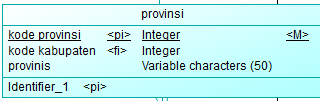
\includegraphics[scale=1.5]{gambar/prov.png}
\caption{\textit{prov}}
\label{prov}
\end{figure}
Dari tabel provinsi tersebut, terdapat kodeprovinsi yang berperan sebagai primary key dengan tipe data integer, tabel ini memiliki atribut lain yaitu provinsi yang memiliki tipe data variable character. Di samping itu, tabel ini memiliki satu foreign key yaitu kodekabupaten dengan tipe data integer yang berasal dari tabel kabupaten.

	\item Tabel Kabupaten\\
\begin{figure}[!htbp]
\centering
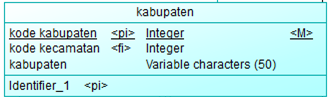
\includegraphics[scale=1.5]{gambar/kab.png}
\caption{\textit{kabupaten}}
\label{kabupaten}
\end{figure}	
	
Tabel Kabupaten  memiliki primary key berupa atribut kodekabupaten dengan tipe data integer dan atribut lain ialah kabupaten dengan tipe data variable character. Tabel kabupaten ini memiliki foreign key berupa atribut kodekecamatan yang bertipe data integer yang berasal dari tabel kecamatan dikarenakan keduanya memiliki hubungan.

	\item Tabel Kecamatan\\
\begin{figure}[!htbp]
\centering
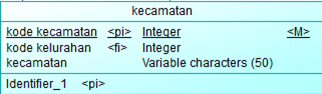
\includegraphics[scale=1.5]{gambar/kec.png}
\caption{\textit{kecamatan}}
\label{kecamatan}
\end{figure}	

Tabel kecamatan tersebut memiliki identifier primary key berupa atribut kodekecamatan yang bertipedata intger, tabel ini memiliki atribut lain yaitu atribut kecamatan dengan tipe data variable character. Tabel kecamatan ini memiliki satu foreign key yaitu kodekelurahan yang bertipe data integer yang berasal dari tabel kelurahan.

\item Tabel Kelurahan\\
\begin{figure}[!htbp]
\centering
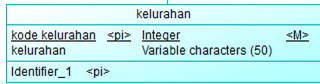
\includegraphics[scale=1.5]{gambar/kel.png}
\caption{\textit{kelurahan}}
\label{kelurahan}
\end{figure}
		Tabel kelurahan tersebut memiliki identifier primary key berupa atribut kodekelurahan yang bertipedata integer dan 1 atribut lain yaitu kelurahan yang memiliki tipe data variable character.

\item Tempat Terbit\\
\begin{figure}[!htbp]
\centering
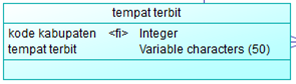
\includegraphics[scale=1.5]{gambar/tempatterbit.png}
\caption{\textit{tempat terbit}}
\label{tmptterbit}
\end{figure}
Tabel tempat terbit tersebut memiliki 1 identifier berupa foreign key yang berasal dari tabel kodekabupaten dengan tipe data integer dan atribut lain yaitu tempat terbit yang berupa variable character.

\item Tanggal Terbit \\
\begin{figure}[!htbp]
\centering
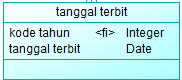
\includegraphics[scale=1.5]{gambar/tglterbit.png}
\caption{\textit{tgl terbit}}
\label{tglterbit}
\end{figure}
Tabel tanggal terbit tersebut memiliki identifier berupa kodetahun yang merupakan primary key dan atribut lain yaitu tanggal terbit yang bertipe data date.
	
	\end{enumerate}
	
\textbf{Kardinalitas}

Jenis-jenis kardinalitas yang digunakan \\
\textbf{one to many} \\
 Setiap baris data dari tabel pertama dapat dihubungkan ke satu baris atau lebih data pada tabel ke dua, contoh : \\	
 \begin{enumerate}
\item 	Relasi antara Tabel agama dan tabel kependudukan\\
yang berarti data dari tabel agama bisa dimiliki oleh 1 atau lebih data dari tabel kependudukan.\\

\item	Relasi antara tabel status perkawinan dengan tabel kependudukan.\\
yang berarti data dari tabel status perkawinan bisa dimiliki oleh 1 atau lebih data dari tabel kependudukan.\\

\item Relasi antara tabel provinsi dengan tabel kependudukan.\\
yang berarti data dari tabel provinsi bisa dimiliki oleh 1 atau lebih data dari tabel kependudukan.\\

\item Relasi antara tabel golongan darah dengan tabel kependudukan.\\
yang berarti data dari tabel golongan darah bisa dimiliki oleh 1 atau lebih data dari tabel kependudukan.\\

\item Relasi antara tabel pekerjaan dengan tabel kependudukan.\\
yang berarti data dari tabel pekerjaan bisa dimiliki oleh 1 atau lebih data dari tabel kependudukan.\\

\item Relasi antara tabel Jenis kelamin dengan tabel kependudukan.\\
yang berarti data dari tabel jenis kelamin bisa dimiliki oleh 1 atau lebih data dari tabel kependudukan.\\

\item Relasi antara tabel tempattanggalterbit dengan tabel kependudukan.\\
yang berarti data dari tabel tempattanggallahir bisa dimiliki oleh 1 atau lebih data dari tabel kependudukan.\\

\item Relasi antara tabel kabupaten dengan tempattanggallahir.\\
yang berarti data dari tabel kabupaten bisa dimiliki oleh 1 atau lebih data dari tabel tempattanggallahir.\\

\item Relasi antara tabel kecamatan dengan tabel kabupaten.\\
yang berarti data dari tabel kabupaten bisa dimiliki oleh 1 atau lebih data dari tabel kecamatan.\\

\item Relasi antara tabel kecamatan dengan tabel kelurahan.\\
yang berarti data dari tabel kecamatan bisa dimiliki oleh 1 atau lebih data dari tabel kelurahan.\\

\item Relasi antara tabel kode pos dengan tabel kecamatan.\\
yang berarti data dari tabel kode pos bisa dimiliki oleh 1 dari tabel kecamatan.\\

\item Relasi antara tabel Kelurahan dengan tabel RT/RW.\\
yang berarti data dari tabel Kelurahan bisa dimiliki oleh 1 atau lebih data dari tabel RT/RW.\\
\end{enumerate}


\begin{figure}[!htbp]
\centering
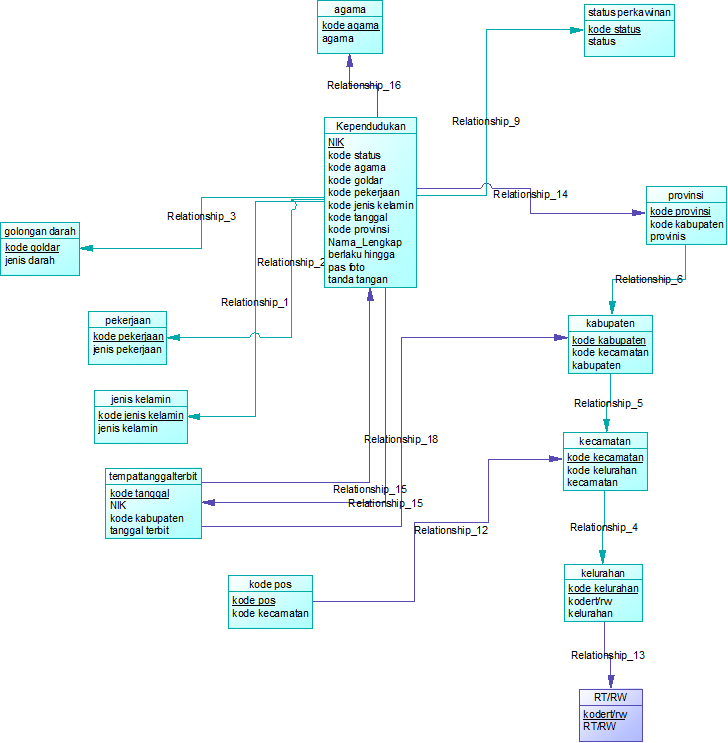
\includegraphics[scale=1.2]{gambar/pdm.png}
\caption{\textit{pdm}}
\label{pdm}
\end{figure}	

\begin{figure}[!htbp]
\centering
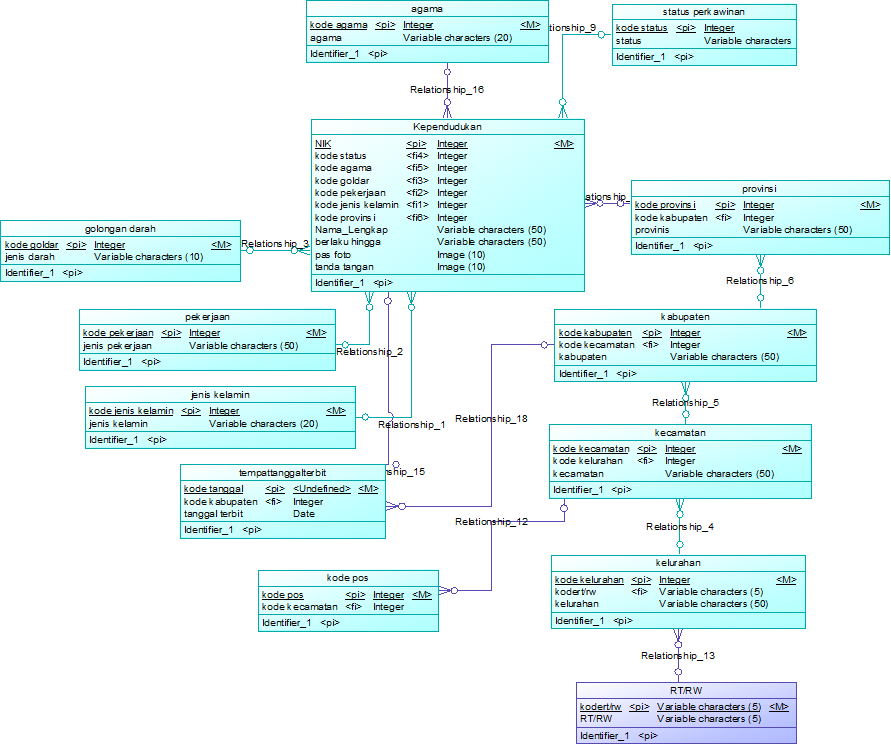
\includegraphics[scale=1.0]{gambar/ldm.png}
\caption{\textit{ldm}}
\label{ldm}
\end{figure}	

\end{document}

